% Generated by Sphinx.
\def\sphinxdocclass{report}
\documentclass[letterpaper,10pt,openany,oneside]{sphinxmanual}
\usepackage[utf8]{inputenc}
\DeclareUnicodeCharacter{00A0}{\nobreakspace}
\usepackage[T1]{fontenc}
\usepackage[english]{babel}
\usepackage{times}
\usepackage[Bjarne]{fncychap}
\usepackage{longtable}
\usepackage{sphinx}
\usepackage{multirow}


\title{Dining Philosophers Documentation}
\date{July 19, 2012}
\release{}
\author{CSInParallel Project}
\newcommand{\sphinxlogo}{}
\renewcommand{\releasename}{}
\makeindex

\makeatletter
\def\PYG@reset{\let\PYG@it=\relax \let\PYG@bf=\relax%
    \let\PYG@ul=\relax \let\PYG@tc=\relax%
    \let\PYG@bc=\relax \let\PYG@ff=\relax}
\def\PYG@tok#1{\csname PYG@tok@#1\endcsname}
\def\PYG@toks#1+{\ifx\relax#1\empty\else%
    \PYG@tok{#1}\expandafter\PYG@toks\fi}
\def\PYG@do#1{\PYG@bc{\PYG@tc{\PYG@ul{%
    \PYG@it{\PYG@bf{\PYG@ff{#1}}}}}}}
\def\PYG#1#2{\PYG@reset\PYG@toks#1+\relax+\PYG@do{#2}}

\def\PYG@tok@gd{\def\PYG@tc##1{\textcolor[rgb]{0.63,0.00,0.00}{##1}}}
\def\PYG@tok@gu{\let\PYG@bf=\textbf\def\PYG@tc##1{\textcolor[rgb]{0.50,0.00,0.50}{##1}}}
\def\PYG@tok@gt{\def\PYG@tc##1{\textcolor[rgb]{0.00,0.25,0.82}{##1}}}
\def\PYG@tok@gs{\let\PYG@bf=\textbf}
\def\PYG@tok@gr{\def\PYG@tc##1{\textcolor[rgb]{1.00,0.00,0.00}{##1}}}
\def\PYG@tok@cm{\let\PYG@it=\textit\def\PYG@tc##1{\textcolor[rgb]{0.25,0.50,0.56}{##1}}}
\def\PYG@tok@vg{\def\PYG@tc##1{\textcolor[rgb]{0.73,0.38,0.84}{##1}}}
\def\PYG@tok@m{\def\PYG@tc##1{\textcolor[rgb]{0.13,0.50,0.31}{##1}}}
\def\PYG@tok@mh{\def\PYG@tc##1{\textcolor[rgb]{0.13,0.50,0.31}{##1}}}
\def\PYG@tok@cs{\def\PYG@tc##1{\textcolor[rgb]{0.25,0.50,0.56}{##1}}\def\PYG@bc##1{\colorbox[rgb]{1.00,0.94,0.94}{##1}}}
\def\PYG@tok@ge{\let\PYG@it=\textit}
\def\PYG@tok@vc{\def\PYG@tc##1{\textcolor[rgb]{0.73,0.38,0.84}{##1}}}
\def\PYG@tok@il{\def\PYG@tc##1{\textcolor[rgb]{0.13,0.50,0.31}{##1}}}
\def\PYG@tok@go{\def\PYG@tc##1{\textcolor[rgb]{0.19,0.19,0.19}{##1}}}
\def\PYG@tok@cp{\def\PYG@tc##1{\textcolor[rgb]{0.00,0.44,0.13}{##1}}}
\def\PYG@tok@gi{\def\PYG@tc##1{\textcolor[rgb]{0.00,0.63,0.00}{##1}}}
\def\PYG@tok@gh{\let\PYG@bf=\textbf\def\PYG@tc##1{\textcolor[rgb]{0.00,0.00,0.50}{##1}}}
\def\PYG@tok@ni{\let\PYG@bf=\textbf\def\PYG@tc##1{\textcolor[rgb]{0.84,0.33,0.22}{##1}}}
\def\PYG@tok@nl{\let\PYG@bf=\textbf\def\PYG@tc##1{\textcolor[rgb]{0.00,0.13,0.44}{##1}}}
\def\PYG@tok@nn{\let\PYG@bf=\textbf\def\PYG@tc##1{\textcolor[rgb]{0.05,0.52,0.71}{##1}}}
\def\PYG@tok@no{\def\PYG@tc##1{\textcolor[rgb]{0.38,0.68,0.84}{##1}}}
\def\PYG@tok@na{\def\PYG@tc##1{\textcolor[rgb]{0.25,0.44,0.63}{##1}}}
\def\PYG@tok@nb{\def\PYG@tc##1{\textcolor[rgb]{0.00,0.44,0.13}{##1}}}
\def\PYG@tok@nc{\let\PYG@bf=\textbf\def\PYG@tc##1{\textcolor[rgb]{0.05,0.52,0.71}{##1}}}
\def\PYG@tok@nd{\let\PYG@bf=\textbf\def\PYG@tc##1{\textcolor[rgb]{0.33,0.33,0.33}{##1}}}
\def\PYG@tok@ne{\def\PYG@tc##1{\textcolor[rgb]{0.00,0.44,0.13}{##1}}}
\def\PYG@tok@nf{\def\PYG@tc##1{\textcolor[rgb]{0.02,0.16,0.49}{##1}}}
\def\PYG@tok@si{\let\PYG@it=\textit\def\PYG@tc##1{\textcolor[rgb]{0.44,0.63,0.82}{##1}}}
\def\PYG@tok@s2{\def\PYG@tc##1{\textcolor[rgb]{0.25,0.44,0.63}{##1}}}
\def\PYG@tok@vi{\def\PYG@tc##1{\textcolor[rgb]{0.73,0.38,0.84}{##1}}}
\def\PYG@tok@nt{\let\PYG@bf=\textbf\def\PYG@tc##1{\textcolor[rgb]{0.02,0.16,0.45}{##1}}}
\def\PYG@tok@nv{\def\PYG@tc##1{\textcolor[rgb]{0.73,0.38,0.84}{##1}}}
\def\PYG@tok@s1{\def\PYG@tc##1{\textcolor[rgb]{0.25,0.44,0.63}{##1}}}
\def\PYG@tok@gp{\let\PYG@bf=\textbf\def\PYG@tc##1{\textcolor[rgb]{0.78,0.36,0.04}{##1}}}
\def\PYG@tok@sh{\def\PYG@tc##1{\textcolor[rgb]{0.25,0.44,0.63}{##1}}}
\def\PYG@tok@ow{\let\PYG@bf=\textbf\def\PYG@tc##1{\textcolor[rgb]{0.00,0.44,0.13}{##1}}}
\def\PYG@tok@sx{\def\PYG@tc##1{\textcolor[rgb]{0.78,0.36,0.04}{##1}}}
\def\PYG@tok@bp{\def\PYG@tc##1{\textcolor[rgb]{0.00,0.44,0.13}{##1}}}
\def\PYG@tok@c1{\let\PYG@it=\textit\def\PYG@tc##1{\textcolor[rgb]{0.25,0.50,0.56}{##1}}}
\def\PYG@tok@kc{\let\PYG@bf=\textbf\def\PYG@tc##1{\textcolor[rgb]{0.00,0.44,0.13}{##1}}}
\def\PYG@tok@c{\let\PYG@it=\textit\def\PYG@tc##1{\textcolor[rgb]{0.25,0.50,0.56}{##1}}}
\def\PYG@tok@mf{\def\PYG@tc##1{\textcolor[rgb]{0.13,0.50,0.31}{##1}}}
\def\PYG@tok@err{\def\PYG@bc##1{\fcolorbox[rgb]{1.00,0.00,0.00}{1,1,1}{##1}}}
\def\PYG@tok@kd{\let\PYG@bf=\textbf\def\PYG@tc##1{\textcolor[rgb]{0.00,0.44,0.13}{##1}}}
\def\PYG@tok@ss{\def\PYG@tc##1{\textcolor[rgb]{0.32,0.47,0.09}{##1}}}
\def\PYG@tok@sr{\def\PYG@tc##1{\textcolor[rgb]{0.14,0.33,0.53}{##1}}}
\def\PYG@tok@mo{\def\PYG@tc##1{\textcolor[rgb]{0.13,0.50,0.31}{##1}}}
\def\PYG@tok@mi{\def\PYG@tc##1{\textcolor[rgb]{0.13,0.50,0.31}{##1}}}
\def\PYG@tok@kn{\let\PYG@bf=\textbf\def\PYG@tc##1{\textcolor[rgb]{0.00,0.44,0.13}{##1}}}
\def\PYG@tok@o{\def\PYG@tc##1{\textcolor[rgb]{0.40,0.40,0.40}{##1}}}
\def\PYG@tok@kr{\let\PYG@bf=\textbf\def\PYG@tc##1{\textcolor[rgb]{0.00,0.44,0.13}{##1}}}
\def\PYG@tok@s{\def\PYG@tc##1{\textcolor[rgb]{0.25,0.44,0.63}{##1}}}
\def\PYG@tok@kp{\def\PYG@tc##1{\textcolor[rgb]{0.00,0.44,0.13}{##1}}}
\def\PYG@tok@w{\def\PYG@tc##1{\textcolor[rgb]{0.73,0.73,0.73}{##1}}}
\def\PYG@tok@kt{\def\PYG@tc##1{\textcolor[rgb]{0.56,0.13,0.00}{##1}}}
\def\PYG@tok@sc{\def\PYG@tc##1{\textcolor[rgb]{0.25,0.44,0.63}{##1}}}
\def\PYG@tok@sb{\def\PYG@tc##1{\textcolor[rgb]{0.25,0.44,0.63}{##1}}}
\def\PYG@tok@k{\let\PYG@bf=\textbf\def\PYG@tc##1{\textcolor[rgb]{0.00,0.44,0.13}{##1}}}
\def\PYG@tok@se{\let\PYG@bf=\textbf\def\PYG@tc##1{\textcolor[rgb]{0.25,0.44,0.63}{##1}}}
\def\PYG@tok@sd{\let\PYG@it=\textit\def\PYG@tc##1{\textcolor[rgb]{0.25,0.44,0.63}{##1}}}

\def\PYGZbs{\char`\\}
\def\PYGZus{\char`\_}
\def\PYGZob{\char`\{}
\def\PYGZcb{\char`\}}
\def\PYGZca{\char`\^}
% for compatibility with earlier versions
\def\PYGZat{@}
\def\PYGZlb{[}
\def\PYGZrb{]}
\makeatother

\begin{document}

\maketitle
\tableofcontents
\phantomsection\label{index::doc}



\chapter{Introduction}
\label{Introduction/Introduction:introduction}\label{Introduction/Introduction::doc}\label{Introduction/Introduction:dining-philosophers}
In this module, you will learn about the Dining Philosophers
Problem and some of the solutions that have been developed for it.
This is a classic problem in concurrency that describes a situation
where multiple processes contend for shared resources. The problem
is originally based on an examination question given by Edsger
Dijkstra in 1965.

Dining Philosophers source file:
\code{dining\_philosophers\_code.tar.gz}


\section{Learning Objectives}
\label{Introduction/Introduction:learning-objectives}\begin{itemize}
\item {} 
Understand the Dining Philosophers Problem and the situations
that it provides a useful model for.

\item {} 
Understand several solutions for the Dining Philosophers problem
and the differences between them.

\item {} 
Be able to implement a simulation in C or C++ that solves the
Dining Philosophers Problem (or at least solves the deadlock
portion of the problem).

\end{itemize}


\section{Requirements}
\label{Introduction/Introduction:requirements}
This module will make use of a number of parallel programming
techniques such as threads (through OpenMP) and message passing
(through OpenMPI). The code provided with this module has only been
tested being compiled with GCC on Linux, although it may work on
other Unix systems. GCC has had support for OpenMP since version
4.2, which was released in 2007. Using OpenMPI requires the OpenMPI
libraries and headers, which can be found in the software the
repositories for many Linux distributions.

In order to run one of the example programs, the OpenMPI
installation needs to have support for multiple threads executing
in the MPI library concurrently. This requires it to be configured
with the \code{-{-}enable-mpi-thread-multiple} option (or
\code{-{-}enable-mpi-threads} for older versions of OpenMPI). To see if
your compilation of OpenMPI supports this feature, the output of
\code{ompi\_info \textbar{} grep Thread} should list \textbf{yes} for
\code{MPI\_THREAD\_MULTIPLE} (or yes for ``mpi'' threads for older
versions of OpenMPI). Note that this only applies to 1 of the 5
example programs.

There are a number of MPI libraries available other than OpenMPI;
it should be possible to use a different one.


\section{Introduction}
\label{Introduction/Introduction:id1}
Suppose that 5 philosophers are sitting around a circular table. A
plate of spaghetti is given to each philosopher, and 5 forks are
distributed around the table so that each philosopher has a left
fork and a right fork that are shared with his neighbors. Each
philosopher independently alternates between thinking and eating.
In order to eat, a philosopher must acquire both his left and right
forks. When done eating, he releases his forks and resumes
thinking. Philosophers are allowed to think for an arbitrary amount
of time, even an infinite amount of time. Philosophers are allowed
to eat for an arbitrary but finite amount of time.

(The problem can also be explained using rice and chopsticks, which
perhaps makes more sense, as it is much harder to eat with one
chopstick than with one fork! We will stick with forks and
spaghetti since it seems to be the more common explanation.)


\section{Requirements for a Solution}
\label{Introduction/Introduction:requirements-for-a-solution}
The philosophers, of course, represent processes or threads running
in a computer, and the forks represent some kind of shared
resource. These shared resources could be a number of things, such
as records in a database or files that can be accessed by only one
process at a time.

We would like to examine the ways that a solution to the Dining
Philosophers problem could be implemented on a real computer or
cluster of computers.

A successful solution to the problem must meet the following
criteria:
\begin{itemize}
\item {} 
Each fork is in use by at most one philosopher at any instant in
time.

\item {} 
All philosophers, upon reaching an hungry state, will be able to
eat within a finite amount of time.

\end{itemize}


\chapter{Shared Memory Dining Philosophers}
\label{SharedMemory/SharedMemory::doc}\label{SharedMemory/SharedMemory:shared-memory-dining-philosophers}
In this section, we consider the case where each philosopher is a
thread. They all share the same memory space.


\section{Observing deadlock}
\label{SharedMemory/SharedMemory:observing-deadlock}
Take a look at the file \code{deadlock.c} in the code distributed with
this module. This is a simple shared memory simulation (but not a
solution!) of the dining philosophers problem. The process is
divided into five threads using an OpenMP parallel section.

\begin{Verbatim}[commandchars=\\\{\}]
	\PYG{c+cm}{/* Each philosopher is a thread */}
\PYG{c+cp}{	\#}\PYG{c+cp}{pragma omp parallel num\PYGZus{}threads(NUM\PYGZus{}PHILOSOPHERS)}
	\PYG{p}{\PYGZob{}}
		\PYG{c+cm}{/* Get the number of this thread and figure out which fork is on}
\PYG{c+cm}{		 * the right and which is on the left. */}
		\PYG{k+kt}{int} \PYG{n}{thread\PYGZus{}num} \PYG{o}{=} \PYG{n}{omp\PYGZus{}get\PYGZus{}thread\PYGZus{}num}\PYG{p}{(}\PYG{p}{)}\PYG{p}{;}
		\PYG{n}{pthread\PYGZus{}mutex\PYGZus{}t} \PYG{o}{*}\PYG{n}{left\PYGZus{}fork} \PYG{o}{=} \PYG{o}{\&}\PYG{n}{forks}\PYG{p}{[}\PYG{n}{thread\PYGZus{}num}\PYG{p}{]}\PYG{p}{;}
		\PYG{n}{pthread\PYGZus{}mutex\PYGZus{}t} \PYG{o}{*}\PYG{n}{right\PYGZus{}fork} \PYG{o}{=} \PYG{o}{\&}\PYG{n}{forks}\PYG{p}{[}\PYG{p}{(}\PYG{n}{thread\PYGZus{}num} \PYG{o}{+} \PYG{l+m+mi}{1}\PYG{p}{)} \PYG{o}{\%} \PYG{n}{NUM\PYGZus{}PHILOSOPHERS}\PYG{p}{]}\PYG{p}{;}

		\PYG{c+cm}{/* Make this thread have a random seed different from the other}
\PYG{c+cm}{		 * threads. */}
		\PYG{k+kt}{unsigned} \PYG{n}{seed} \PYG{o}{=} \PYG{n}{t} \PYG{o}{+} \PYG{n}{thread\PYGZus{}num}\PYG{p}{;}
		\PYG{k}{while} \PYG{p}{(}\PYG{l+m+mi}{1}\PYG{p}{)} \PYG{p}{\PYGZob{}}
			\PYG{n}{philosopher\PYGZus{}cycle}\PYG{p}{(}\PYG{n}{thread\PYGZus{}num}\PYG{p}{,} \PYG{n}{left\PYGZus{}fork}\PYG{p}{,} \PYG{n}{right\PYGZus{}fork}\PYG{p}{,} \PYG{o}{\&}\PYG{n}{seed}\PYG{p}{)}\PYG{p}{;}
		\PYG{p}{\PYGZcb{}}
	\PYG{p}{\PYGZcb{}}
\end{Verbatim}

OpenMP (which stands for Open Multi-Processing) is an API that makes it
easier to write multithreaded programs in C, C++, and Fortran. It
works mainly by using \textbf{pragmas}, directives that give information
to the compiler. It also offers a number of functions such as
\code{omp\_get\_thread\_num()}. To use OpenMP in a C or C++
program, you must pass the flag \code{-fopenmp} to GCC. This flag must
be specified both for the compilation phase, so that the OpenMP
pragmas are interpreted, and for the linking phase, so that the
programs are linked with \code{libgomp}, the GNU implementation of the
OpenMP API (which is part of gcc). Also, if any OpenMP functions
are called explicitly, \code{omp.h} must be included.

The forks are represented by \textbf{mutexes}. These are program objects
that can only be modified by one thread at a time -- that is,
modifying them is an atomic operation.

\begin{Verbatim}[commandchars=\\\{\}]
	\PYG{c+cm}{/* The forks are represented by an array of mutexes. */}
	\PYG{n}{pthread\PYGZus{}mutex\PYGZus{}t} \PYG{n}{forks}\PYG{p}{[}\PYG{n}{NUM\PYGZus{}PHILOSOPHERS}\PYG{p}{]}\PYG{p}{;}
\end{Verbatim}

More specifically, a mutex is a special case of a \textbf{semaphore},
an object that allows atomic increment and decrement operations. A mutex is a
\textbf{binary semaphore} that only allows two values. These two states
can be referred to as ``locked'' and ``unlocked'' A mutex can be used
to ensure exclusive access to objects or sections of code because
only one thread can have locked the mutex at a time.

Each thread (philosopher) enters a loop in which it thinks and
eats.

\begin{Verbatim}[commandchars=\\\{\}]
\PYG{c+cm}{/* Called each time a philosopher wants to eat. */}
\PYG{k}{static} \PYG{k+kt}{void} \PYG{n+nf}{philosopher\PYGZus{}cycle}\PYG{p}{(}\PYG{k+kt}{int} \PYG{n}{thread\PYGZus{}num}\PYG{p}{,} \PYG{n}{pthread\PYGZus{}mutex\PYGZus{}t} \PYG{o}{*}\PYG{n}{left\PYGZus{}fork}\PYG{p}{,} 
		\PYG{n}{pthread\PYGZus{}mutex\PYGZus{}t} \PYG{o}{*}\PYG{n}{right\PYGZus{}fork}\PYG{p}{,} \PYG{k+kt}{unsigned} \PYG{o}{*}\PYG{n}{seed}\PYG{p}{)}
\PYG{p}{\PYGZob{}}
	\PYG{n}{printf}\PYG{p}{(}\PYG{l+s}{"}\PYG{l+s}{Philosopher \%d wants to eat!}\PYG{l+s+se}{\PYGZbs{}n}\PYG{l+s}{"}\PYG{p}{,} \PYG{n}{thread\PYGZus{}num}\PYG{p}{)}\PYG{p}{;}

	\PYG{n}{pthread\PYGZus{}mutex\PYGZus{}lock}\PYG{p}{(}\PYG{n}{left\PYGZus{}fork}\PYG{p}{)}\PYG{p}{;}
	\PYG{n}{printf}\PYG{p}{(}\PYG{l+s}{"}\PYG{l+s}{Philosopher \%d picked up his left fork.}\PYG{l+s+se}{\PYGZbs{}n}\PYG{l+s}{"}\PYG{p}{,} \PYG{n}{thread\PYGZus{}num}\PYG{p}{)}\PYG{p}{;}
	\PYG{n}{pthread\PYGZus{}mutex\PYGZus{}lock}\PYG{p}{(}\PYG{n}{right\PYGZus{}fork}\PYG{p}{)}\PYG{p}{;}
	\PYG{n}{printf}\PYG{p}{(}\PYG{l+s}{"}\PYG{l+s}{Philosopher \%d picked up his right fork and }\PYG{l+s}{"}
			\PYG{l+s}{"}\PYG{l+s}{started eating.}\PYG{l+s+se}{\PYGZbs{}n}\PYG{l+s}{"}\PYG{p}{,} \PYG{n}{thread\PYGZus{}num}\PYG{p}{)}\PYG{p}{;}

	\PYG{n}{sleep\PYGZus{}rand\PYGZus{}r}\PYG{p}{(}\PYG{n}{min\PYGZus{}eat\PYGZus{}ms}\PYG{p}{[}\PYG{n}{thread\PYGZus{}num}\PYG{p}{]}\PYG{p}{,} \PYG{n}{max\PYGZus{}eat\PYGZus{}ms}\PYG{p}{[}\PYG{n}{thread\PYGZus{}num}\PYG{p}{]}\PYG{p}{,} \PYG{n}{seed}\PYG{p}{)}\PYG{p}{;}

	\PYG{n}{pthread\PYGZus{}mutex\PYGZus{}unlock}\PYG{p}{(}\PYG{n}{left\PYGZus{}fork}\PYG{p}{)}\PYG{p}{;}
	\PYG{n}{pthread\PYGZus{}mutex\PYGZus{}unlock}\PYG{p}{(}\PYG{n}{right\PYGZus{}fork}\PYG{p}{)}\PYG{p}{;}
	\PYG{n}{printf}\PYG{p}{(}\PYG{l+s}{"}\PYG{l+s}{Philosopher \%d is done eating and has released his }\PYG{l+s}{"}
			\PYG{l+s}{"}\PYG{l+s}{forks.}\PYG{l+s+se}{\PYGZbs{}n}\PYG{l+s}{"}\PYG{p}{,} \PYG{n}{thread\PYGZus{}num}\PYG{p}{)}\PYG{p}{;}

	\PYG{n}{sleep\PYGZus{}rand\PYGZus{}r}\PYG{p}{(}\PYG{n}{min\PYGZus{}think\PYGZus{}ms}\PYG{p}{[}\PYG{n}{thread\PYGZus{}num}\PYG{p}{]}\PYG{p}{,} \PYG{n}{max\PYGZus{}think\PYGZus{}ms}\PYG{p}{[}\PYG{n}{thread\PYGZus{}num}\PYG{p}{]}\PYG{p}{,} \PYG{n}{seed}\PYG{p}{)}\PYG{p}{;}
\PYG{p}{\PYGZcb{}}
\end{Verbatim}

A \textbf{reentrant} function-- that is, a function that returns
consistent results when called by multiple threads concurrently--
that sleeps the calling thread for a random number of milliseconds
is defined to implement the ``thinking'' and ``eating''.
\begin{figure}[htbp]
\centering
\capstart

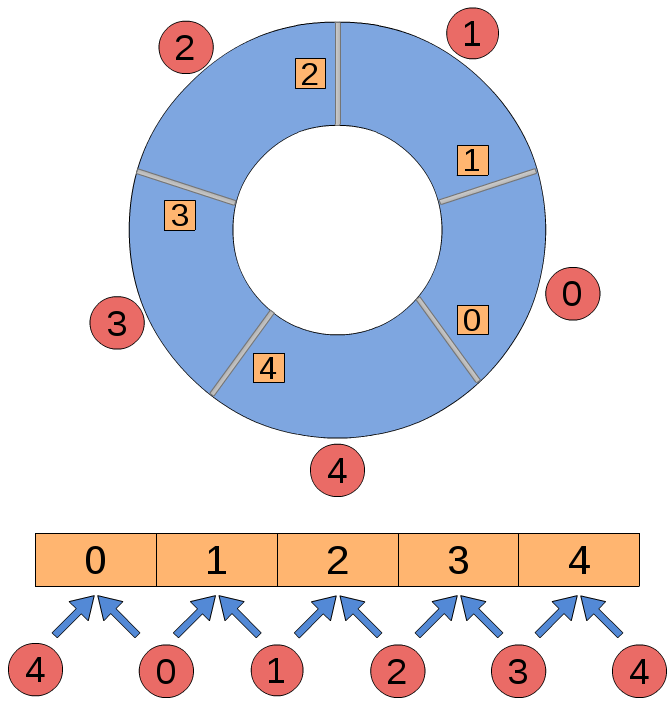
\includegraphics{Figure1.png}
\caption{Figure 1. In this figure, red circles represent philosophers, or threads. Orange rectangulars represent forks, or common resource that threads are sharing.}\end{figure}

Compile \code{deadlock.c} using \code{make deadlock} (or just type \code{make}
to compile all the examples at once), then run it. Observe the
simulation for a while before interrupting it.

Did you notice any problems? Most likely not, if you ran the
simulation for only a short period of time. There is a major
problem with the code though. In the function \emph{philosopher\_cycle},
try adding a very short delay between the time the philosophers
pick up their left fork and the time the philosophers pick up their
right fork, like this:

\begin{Verbatim}[commandchars=\\\{\}]
\PYG{n}{pthread\PYGZus{}mutex\PYGZus{}lock}\PYG{p}{(}\PYG{n}{left\PYGZus{}fork}\PYG{p}{)}\PYG{p}{;}
\PYG{n}{printf}\PYG{p}{(}\PYG{l+s}{"}\PYG{l+s}{Philosopher }\PYG{l+s+si}{\%d}\PYG{l+s}{ picked up his left fork.}\PYG{l+s+se}{\PYGZbs{}n}\PYG{l+s}{"}\PYG{p}{,} \PYG{n}{thread\PYGZus{}num}\PYG{p}{)}\PYG{p}{;}
\PYG{n}{millisleep}\PYG{p}{(}\PYG{l+m+mi}{5}\PYG{p}{)}\PYG{p}{;}
\PYG{n}{pthread\PYGZus{}mutex\PYGZus{}lock}\PYG{p}{(}\PYG{n}{right\PYGZus{}fork}\PYG{p}{)}\PYG{p}{;}
\end{Verbatim}

Now try running the code again. What happens?

Most likely all the philosophers picked up their left fork, at
which point they all became permanently \textbf{deadlocked} because each
philosopher was waiting on each other in turn. All the threads were
waiting for a resource that will never be released.

This problem can only occur if 4 of the 5 threads are preempted
after picking up their left fork but before picking up their right
fork. This is unlikely to occur without a delay between the locks.
But even so, the possibility of deadlock is a major flaw in this
code. After all, you wouldn't want to use an operating system or
program that could lock up at any time!


\section{A ``Solution'' that avoids deadlock}
\label{SharedMemory/SharedMemory:a-solution-that-avoids-deadlock}
Is there a simple way to prevent deadlock from occurring?

Suppose that not all of the philosophers were to pick up their
forks in the same order. That is, some of the philosophers would
pick up their forks left-right, and others would pick up their
forks right-left. This would therefore be an asymmetrical solution,
since not all of the philosophers would act in the same way.

It turns out that deadlock will be avoided simply if the fifth
philosopher picks up his forks in the opposite order from everyone
else. If the first four philosophers have all picked up their left
fork, then the fifth philosopher will be unable to pick up the last
fork, since it would be his second fork to pick up. Similarly, if
the fifth philosopher is holding one fork, then it is impossible
for the first philosopher to pick up any forks. It is therefore
guaranteed that deadlock will not occur.

Compile and run \code{partial\_order.c}.

\begin{Verbatim}[commandchars=\\\{\}]
	\PYG{k}{if} \PYG{p}{(}\PYG{n}{thread\PYGZus{}num} \PYG{o}{=}\PYG{o}{=} \PYG{n}{NUM\PYGZus{}PHILOSOPHERS} \PYG{o}{-} \PYG{l+m+mi}{1}\PYG{p}{)} \PYG{p}{\PYGZob{}}
		\PYG{n}{pthread\PYGZus{}mutex\PYGZus{}lock}\PYG{p}{(}\PYG{n}{right\PYGZus{}fork}\PYG{p}{)}\PYG{p}{;}
		\PYG{n}{printf}\PYG{p}{(}\PYG{l+s}{"}\PYG{l+s}{Philosopher \%d picked up his right fork.}\PYG{l+s+se}{\PYGZbs{}n}\PYG{l+s}{"}\PYG{p}{,} \PYG{n}{thread\PYGZus{}num}\PYG{p}{)}\PYG{p}{;}
		\PYG{n}{millisleep}\PYG{p}{(}\PYG{l+m+mi}{5}\PYG{p}{)}\PYG{p}{;}
		\PYG{n}{pthread\PYGZus{}mutex\PYGZus{}lock}\PYG{p}{(}\PYG{n}{left\PYGZus{}fork}\PYG{p}{)}\PYG{p}{;}
		\PYG{n}{printf}\PYG{p}{(}\PYG{l+s}{"}\PYG{l+s}{Philosopher \%d picked up his left fork and }\PYG{l+s}{"}
				\PYG{l+s}{"}\PYG{l+s}{started eating.}\PYG{l+s+se}{\PYGZbs{}n}\PYG{l+s}{"}\PYG{p}{,} \PYG{n}{thread\PYGZus{}num}\PYG{p}{)}\PYG{p}{;}
	\PYG{p}{\PYGZcb{}} \PYG{k}{else} \PYG{p}{\PYGZob{}}
		\PYG{n}{pthread\PYGZus{}mutex\PYGZus{}lock}\PYG{p}{(}\PYG{n}{left\PYGZus{}fork}\PYG{p}{)}\PYG{p}{;}
		\PYG{n}{printf}\PYG{p}{(}\PYG{l+s}{"}\PYG{l+s}{Philosopher \%d picked up his left fork.}\PYG{l+s+se}{\PYGZbs{}n}\PYG{l+s}{"}\PYG{p}{,} \PYG{n}{thread\PYGZus{}num}\PYG{p}{)}\PYG{p}{;}
		\PYG{n}{millisleep}\PYG{p}{(}\PYG{l+m+mi}{5}\PYG{p}{)}\PYG{p}{;}
		\PYG{n}{pthread\PYGZus{}mutex\PYGZus{}lock}\PYG{p}{(}\PYG{n}{right\PYGZus{}fork}\PYG{p}{)}\PYG{p}{;}
		\PYG{n}{printf}\PYG{p}{(}\PYG{l+s}{"}\PYG{l+s}{Philosopher \%d picked up his right fork and }\PYG{l+s}{"}
				\PYG{l+s}{"}\PYG{l+s}{started eating.}\PYG{l+s+se}{\PYGZbs{}n}\PYG{l+s}{"}\PYG{p}{,} \PYG{n}{thread\PYGZus{}num}\PYG{p}{)}\PYG{p}{;}
	\PYG{p}{\PYGZcb{}}
\end{Verbatim}

It is very similar to
\code{deadlock.c}, but it adds in a simple if-else statement around
the code where the philosophers pick up their forks, so that the
last philosopher picks up his forks in the opposite order from the
others. A delay between picking up the two forks has already been
added. You will see that this code will not deadlock.

This solution can be generalized to the idea of assigning a partial
order to the resources. In the classic dining philosophers problem,
the forks would be numbered from 0 to 4. In this situation,
processes must acquire their resources in order from lowest to
highest. This will work for any number of processes acquiring any
number of resources. However, if the needed resources are not known
in advance, this can be an inconvenient solution; this is because
if a process has decided it needs a resource after it has already
acquired higher numbered resources, it must release the higher
numbered resources first, acquire the needed resource, then
reacquire the released resources in order.


\section{Starvation}
\label{SharedMemory/SharedMemory:starvation}
There is still a problem with the solution in \code{partial\_order.c,
however. Take a look at the code in {}`{}`partial\_order2.c}. This is
similar to the original \code{partial\_order.c}, but an interrupt
handler has been added. This interrupt handler prints out the
number of times each philosopher has eaten when the program is
interrupted (when Control-C is pressed). The philosophers also
think and eat much faster and have no delay between acquiring the
forks.

Compile \code{partial\_order\_2.c}, then let it run for a little
while before interrupting it. Look at how many times each
philosopher has eaten and thought. Are they about the same? Or does
it look like some philosophers had an advantage over others?

Your results will vary, but here are our results after running the
simulation for a few minutes:

\begin{tabulary}{\linewidth}{|L|L|}
\hline
\textbf{
Philosopher
} & \textbf{
Times Eaten
}\\\hline

Philsopher 0:
 & 
4341 times eaten
\\\hline

Philsopher 1:
 & 
4529 times eaten
\\\hline

Philsopher 2:
 & 
4612 times eaten
\\\hline

Philsopher 3:
 & 
4673 times eaten
\\\hline

Philsopher 4:
 & 
4340 times eaten
\\\hline
\end{tabulary}


Philosopher 4 and 0 appear to eat and think less often than the
other philosophers; thus, they spend more time in the ``hungry''
state, waiting to acquire forks.

This imperfection is a result of the asymmetry of the solution:
since not all the philosophers are acting in the same way, it is
possible that some philosophers do not have the same chance to eat
as others do.

If you think about it, you may realize there is a more fundamental
problem as well. Suppose that philosopher 2 wants to eat, but
philosophers 1 and 3 are currently eating. Philosopher 2's thread
is put to sleep as it waits for the forks. Meanwhile, philosophers
1 and 3 finish eating, but philosopher 2's thread is not scheduled
to run right away. Rather, before philosopher 2's thread is run
again, philosophers 1 and 3 start to eat again. Philosopher 2 never
had a chance to eat! What if this keeps happening over and over?

The problem here is that one of the philosophers could potentially
``starve'' because of a timing problem. This is independent from the
possibility of deadlock, which has already been eliminated in the
partial order solution.

We will return to the starvation problem later when we discuss the
Chandry-Misra solution.


\chapter{Distributed Dining Philosophers}
\label{Distributed/Distributed:distributed-dining-philosophers}\label{Distributed/Distributed::doc}

\section{OpenMPI}
\label{Distributed/Distributed:openmpi}
In this section we discuss the Dining Philosophers problem where
each philosopher is a separate process. Memory is not shared. We
make use of \textbf{OpenMPI}, an implementation of \textbf{MPI}, which stands
for \textbf{Message Passing Interface}. OpenMPI provides an API for
sending data from one process to another. Programs using OpenMPI
must include \code{mpi.h} and link with a number of libraries. You can
use the wrapper compiler \code{mpicc} to avoid having to specify all
the MPI libraries when linking your program.

MPI programs are run by using the \code{mpirun} command. This command
allows you to specify the number of processes to start and which
hosts to start them on. Although the processes may or may not run
on different hosts, in the program code itself there is no
difference between sending data to a process running on the same
computer and sending data to a process running on a different
computer. This is because OpenMPI provides the concept of a
``communicator'' containing a number of processes, where each process
has a number. To send a message to a process, you simply need to
specify its number and communicator.

OpenMPI supports both blocking and unblocking sends and receives.
Blocking sends and receives, such as \code{MPI\_Send()} and
\code{MPI\_Recv()}, block until the message is actually send or
received, while nonblocking sends and receives, such as
\code{MPI\_Isend()} and \code{MPI\_Irecv()}, return immediately. If using
nonblocking message passing, you can later test to see if a message
has completed using the \code{MPI\_Test()} class of functions or wait
for a message to complete using the \code{MPI\_Wait()} class of
functions. If you have installed the OpenMPI documentation, there
should be a man page on each MPI function.


\section{A ``Waiter'' solution to the distributed Dining Philosophers problem}
\label{Distributed/Distributed:a-waiter-solution-to-the-distributed-dining-philosophers-problem}
One of the simplest solutions to resource management problems like
the Dining Philosophers problem is to centralize the problem by
having a master thread or master process that determines which
threads or processes are able to access resources. For the Dining
Philosophers problem, this can be called the \textbf{waiter} solution.

In order to solve the dining philosophers problem in a distributed
manner using the waiter solution, the philosopher processes must
communicate with the waiter using message passing. That is, they
must ask for permission to eat, and the waiter, who has control of
all the forks, decides who gets to eat and sends them a message
telling them to go ahead.

The waiter may only be concerned with preventing deadlock, or he
may also keep track of which philosophers have eaten and give an
advantage to philosophers who are starving.

In the file \code{distributed\_waiter.c}, there is an implementation
of the waiter solution to the distributed dining philosophers
problem. It is not a full solution, since it only solves the
deadlock problem and not the starvation problem. Take a look at the
code and read the comments to try to understand it. Support for MPI
threads is not needed to run this program as it only uses
processes, not threads.

Since the waiter is its own process, \code{distributed\_waiter} must be
run using 6 processes in order to simulate 5 philosophers.


\section{The Chandry-Misra solution to the distributed Dining Philosophers problem}
\label{Distributed/Distributed:the-chandry-misra-solution-to-the-distributed-dining-philosophers-problem}
Although having a waiter process can fully solve the dining
philosophers problem, the disadvantage is that all philosophers
have to wait for the one waiter, who could be overloaded with work
if there are too many philosophers. Is it possible to solve the
dining philosophers problem in a distributed, decentralized
manner?

In 1984, K. M. Chandry and J. Misra published a paper titled
\emph{The drinking philosophers problem} \footnote{\begin{enumerate}
\setcounter{enumi}{10}
\item {} \begin{enumerate}
\setcounter{enumi}{12}
\item {} 
Chandry and J. Misra. The drinking philosophers problem. ACM Transactions on Programming Languages and Systems, 6(4):632–646, October 1984.

\end{enumerate}

\end{enumerate}
}. In it, they
provide a completely distributed solution to the Dining
Philosophers problem that avoids both deadlock and starvation. They
also generalize their solution to what they call the
``Drinking Philosophers problem'', where an arbitrary number of
agents can share any number of resources (``bottles'') with other
agents and require any number of these resources for each
``drinking'' session.

For the full details of their solution, you should see their
original paper, which as of this writing is freely available
online. We will give you a summary of their solution and show you
some code that implements it.

In Chandry and Misra's solution to the Dining Philosophers problem,
idea of the forks being \emph{clean} and \emph{dirty} is introduced. The
solution is completely distributed, and philosophers must send
``request tokens'' to other philosophers to request their forks.
``Dirty'' forks must be given up if they are requested, while ``clean''
forks may be kept, unless they are not needed. Whenever a fork is
used to eat, it becomes dirty, and whenever a fork is sent to
another philosopher, it is cleaned (if it is not already clean).

The deadlock problem is solved by ensuring that no cycles can
develop in the precedence graph that represents which philosophers
have priorities over others. Additionally, the starvation problem
is solved because the cleanliness of the forks will ensure that any
one philosopher will not wait forever to eat.

In the file \code{chandry\_misra.c}, there is an implementation of
this solution. Messages are passed between processes using OpenMPI.
Read some of the comments in the code to better understand the
solution.

In order to run this program, the MPI library must support multiple
threads executing in the MPI library concurrently. This is because
each philosopher process is divided into 2 threads: a main thread
that does the thinking and eating, and a helper thread that listens
for requests for forks from the philosophers' neighbors at all
times, including when the main thread is thinking. This design is
necessary if we do not allow for the possibility that forks can be
owned by no philosophers. If at any point in time, the fork must be
held by one of the two philosophers or be in transit between the
two, it cannot be guaranteed that the other philosopher can get the
fork if one philosopher decides to think for an arbitrarily long
period of time, during which he cannot release the fork-- but the
Chandry-Misra solution requires that he does in fact release the
fork somehow. The helper thread solves this problem by allowing the
philosopher's forks to be given up while he is thinking.

Run the program with \code{mpirun -n 5 chandry\_misra {[}SECONDS{]}}. The
default number of seconds to run the simulation for is 5.
Statistics are shown when the simulation finishes. The default
eating and thinking times are set to be very fast, but you can
adjust this in the arrays near the top of the code. Try running the
code for a hundred seconds or so and look at the results. Does it
look like all the philosophers had an equal chance to eat? You will
be able to tell from the results, although they won't be able to
tell you if starvation is theoretically possible. But the solution
does, in fact, guarantee that each any every philosopher will be
able to eat within a finite amount of time once he becomes hungry.



\renewcommand{\indexname}{Index}
\printindex
\end{document}
